\documentclass{article}

\usepackage{geometry}
\usepackage{amsmath, amsfonts, amsthm}
\usepackage{algorithm, algpseudocode}
\usepackage{graphicx, subcaption, float}

\graphicspath{{./images/}}

\newcommand{\tskit}{{\texttt{tskit}}}
\newcommand{\tsinfer}{{\texttt{tsinfer}}}
\newcommand{\msprime}{{\texttt{msprime}}}
\newcommand{\twisst}{{\textit{TWISST}}}

\begin{document}

\title{Efficiently Computing Species Trees Distributions Along the Genome}
\author{Daniel Goldstein}
\maketitle


\section{Introduction}

The inference of species trees from genomic data is a fundamental problem in
evolutionary biology. They reveal the relatedness between species and broaden 
our understanding of evolutionary processes. However, there is not generally
only one species tree that can describe a set of samples.
Processes like admixture can create genetic sequences that reflect
alternate species trees.
Genetic events like recombination can cause different regions of the genome
to reflect different species histories within the same sample.
So instead of a single species tree we must consider a distribution
of likelihoods over all possible topologies for every position on the genome.
Inferring these distributions from variant data often requires complex
statistical models and are expensive to compute across large sequences.
Here, we discuss a simple approach for computing exact
species tree distributions that relies on the tree sequence data model.
Using tree sequences, we can compute these results in record time and
scale well in terms of sample size and sequence length.

Tree sequences are a lossless, efficient method of storing and processing
variant data that leverages the shared genetic material between samples.
Samples are represented as leaves in ancestral trees that span
particular intervals of the genome. The high correlation between adjacent
trees in the sequence allows us to store the minimal information to transform
one tree into the next, instead of storing each tree independently. This
significantly decreases storage space and yields an efficient way to iterate
through the data. Using this form iteration, we can design tree sequence
algorithms to recompute only the necessary information required to calculate
the result for the following tree.
This approach is called an incremental algorithm and is the reason this
we can quickly compute species trees distributions for tens of thousands of
trees along the genome.

\section{Method}
\subsection{Ranking tree topologies}

Before we can discuss the algorithm for calculating a species trees, we
need a system to refer to and identify them uniquely.
In the context of this method, we require that species trees be rooted,
leaf-labelled trees with no unary nodes.
Since there exists a finite number of topologies under this definition
of equality, we can use a combinatorial approach to index, or rank,
tree topologies.
This rank serves as a reversible hash on species trees, meaning we can
easily convert back and forth between a tree representation and its
rank among all possible species trees. The rank is used in the following
algorithms to count occurences of unique species tree topologies.

\subsection{Species trees distributions on a single tree}

The method for computing species trees distributions is inspired by the method
\twisst, which works
by repetitively selecting samples, one from each species, and tracing the
embedded tree that they form within the larger gene tree. Taking each
sample to represent the species from which it was chosen, we identify
the species tree topology reflected by that single sample combination.
Tallying the number of sample combinations that
reflect each unique topology gives a distribution of species trees
embedded in the single gene tree. By exhausting all sample combinations,
we obtain an exact distribution.

However, this approach scales poorly with sample size as the number
of sample combinations for $n$ samples and $p$ populations is $O(n^p)$ for
$p \ll n$. Approximations can be obtained by running a set number of iterations
but at the cost of needing to choose a fair subset of sample combinations and
accounting for this approximation downstream.

Our method uses a dynamic programming approach to reduce the algorithmic
complexity to be linear in $n$, while also producing an exact distribution.
The approach relies on the following points:
\begin{enumerate}
    % What is the name of a leaf root?
    \item A leaf root contains a single species tree: that of the species to
        which the sample belongs.
    \item An internal node contains the species trees of its children, as
        well as all combinations of trees from its children whose
        sets of species are disjoint.
\end{enumerate}
These rules yield a single-pass algorithm from the leaves of the tree
up to the root. Figure~\ref{fig:dp_alg} and Algorithm~\ref{alg:dp_alg}
illustrate this in the case of binary trees, but the same approach generalizes
to trees with any number of polytomies.

\begin{figure}[H]
    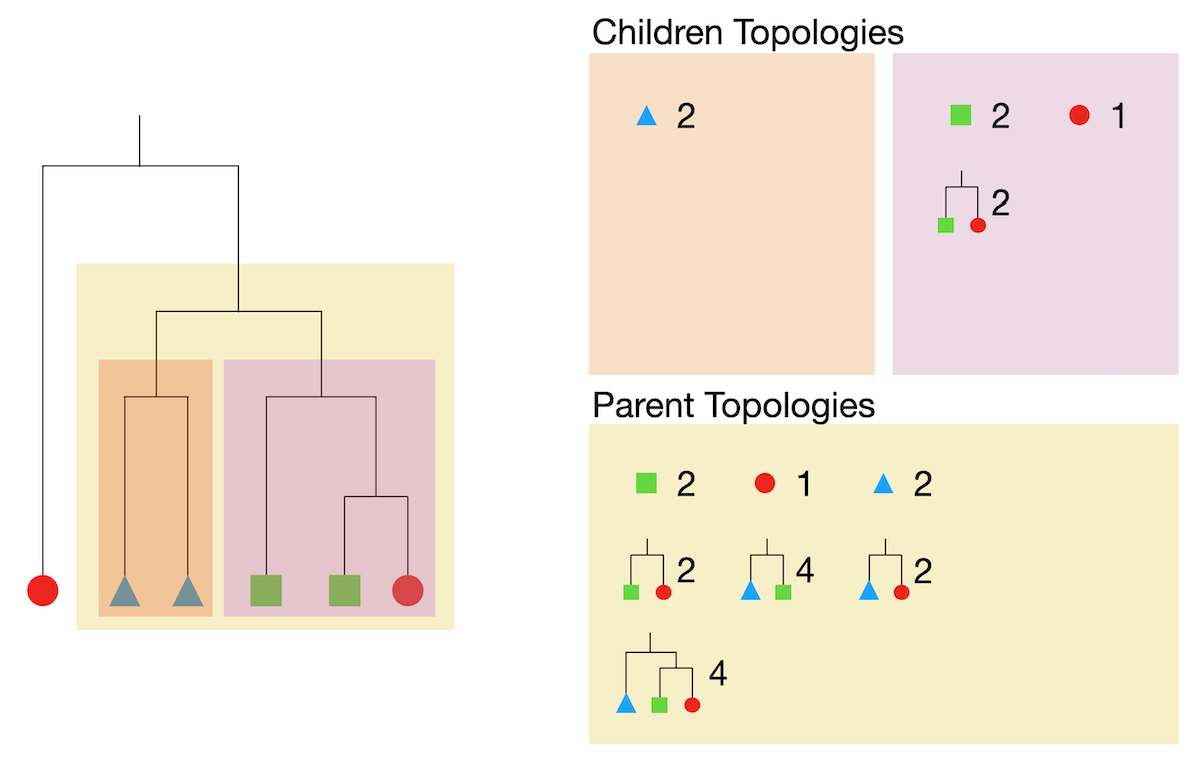
\includegraphics[scale=0.5]{dp_alg}
    \centering
    \caption{Counting embedded species trees at an internal node}
    \label{fig:dp_alg}
\end{figure}

The algorithm state at each node is the unique topologies,
represented by their ranks, embedded in the subtree under that node, and the
counts of how many times each topology is represented in the subtree. This
limits the size of the state to the number of unique species tree topologies,
not the number of samples. At an internal node $u$, we perform a cartesian
product of the states of $u$'s children to discover disjoint species trees that
can be combined under $u$.

\begin{algorithm}
\label{alg:dp_alg}
    \caption{Computing species tree topologies in a single gene tree}
    \begin{algorithmic}
        \State state = []

        \ForAll{$u$ in leaves}
        \State state[$u$] $\leftarrow$ \{(species(u)): 0\} // The rank of a root leaf is 0
        \EndFor

        \ForAll{$u$ in postorder internal nodes}
            \State topologies = \{\}
            \State topologies $\leftarrow$ propagate child topologies // TODO
            \State topologies $\leftarrow$ join disjoint child topologies // TODO
            \State state[$u$] = topologies
        \EndFor
        \State \Return state[root]
    \end{algorithmic}
\end{algorithm}
If we let $t(p)$ be the number of unique tree topologies with $p$ leaves,
we get that the algorithmic complexity is
\[
    O(n \big(\sum_{i=1}^p t(i)\big)^2) = O(n t(p)^2)
\]
since $t(p)$ grows factorially in $p$. We know however that $p \ll n$, so is
dominated by a runtime linear in $n$.

This algorithm also has the nice property that it works on gene trees
that have not completely coalesced. Instead of the final result being
\texttt{state[root]}, we simply take the union of the topology distributions
from each root.

\subsection{Spanning a genome}
This algorithm works well for a single tree, but does not scale when multiplied
across tens or hundreds of thousands of trees as is typical in a tree sequence.
Fortunately, the substructure property allows us to reuse state between trees
where the subtree under a node is unaffected by a tree transition.
As we transition from one tree to the next, instead of constructing
the next tree from scratch we perform a Subtree-Prune-and-Regraft (SPR) operation
on the current tree to obtain the next.
When a node $u$ is removed or inserted into the tree during an SPR, we do not
need to compute the topologies within the subtree.
Instead we need only ``pick up'' the previous algorithm at $u$ and traverse
upward toward the root.
Since there is a constant number of edges removed and inserted between trees
in a tree sequence, this process takes only $O(\log(n)t(p)^2)$ time.

\section{Discussion}
We test this functionality by examining a \msprime{} simulation in which we've simulated
25 thousand 1mb genomes distributed evenly between four species: orangutan,
gorilla, chimp and human. This produced a \tskit{} tree sequence with
31 thousand trees. Figure~\ref{fig:great_apes} ilustrates the four unique
species tree topologies represented in the tree sequence, the positions
along the sequence they were observed, and the frequency of each.

\begin{figure}[H]
    \begin{minipage}{.48\textwidth}
        \begin{subfigure}{\linewidth}
            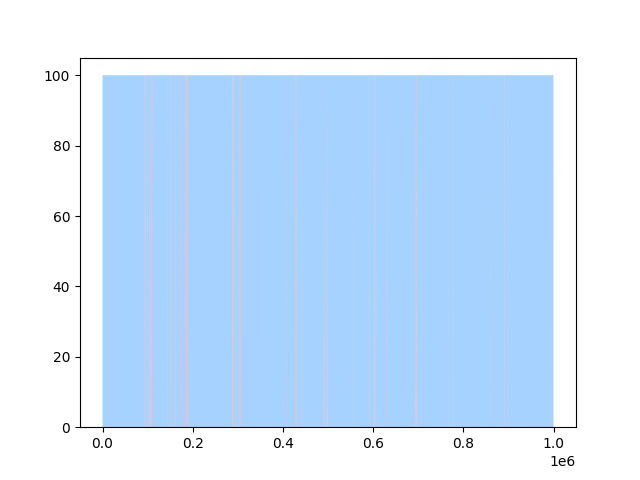
\includegraphics[scale=0.48]{great_apes_area_plot.png}
        \end{subfigure}
    \end{minipage}
    \begin{minipage}{.48\textwidth}
        \begin{minipage}{.4\textwidth}
            \begin{subfigure}[b]{\linewidth}
                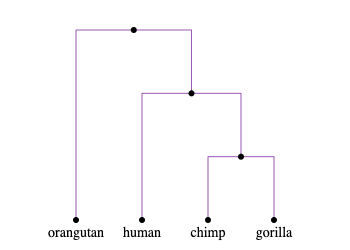
\includegraphics[scale=0.3]{tree_0.png}
                \subcaption{1.79\% weighted}
            \end{subfigure}
            \begin{subfigure}[b]{\linewidth}
                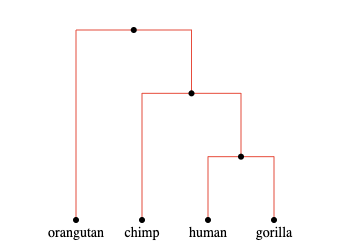
\includegraphics[scale=0.3]{tree_1.png}
                \subcaption{1.79\% weighted}
            \end{subfigure}
        \end{minipage}
        \begin{minipage}{.4\textwidth}
            \begin{subfigure}[b]{\linewidth}
                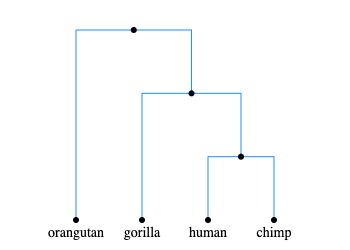
\includegraphics[scale=0.3]{tree_2.png}
                \subcaption{96.41\% weighted}
            \end{subfigure}
            \begin{subfigure}[b]{\linewidth}
                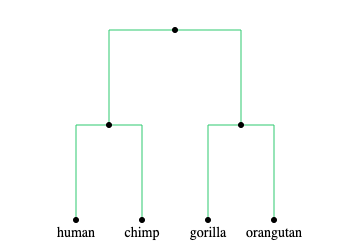
\includegraphics[scale=0.3]{tree_3.png}
                \subcaption{0.01\% weighted}
            \end{subfigure}
        \end{minipage}
    \end{minipage}
    \centering
    \caption{Great apes simulation species trees across the genome}
    \label{fig:great_apes}
\end{figure}

The performance benefits of using an incremental approach is evident when
examining the time taken per tree. Computing Algorithm~\ref{alg:dp_alg}
took just over 1.4 seconds as it computed the topologies for every node in
the 25 thousand leaf tree. For subsequent trees, however, only partial
applications of the algorithm must be made to update species topologies, and
\tskit{} is able to process over 130 trees per second, resulting in an overall
runtime of 4 minutes and 28 seconds.

\begin{figure}[H]
    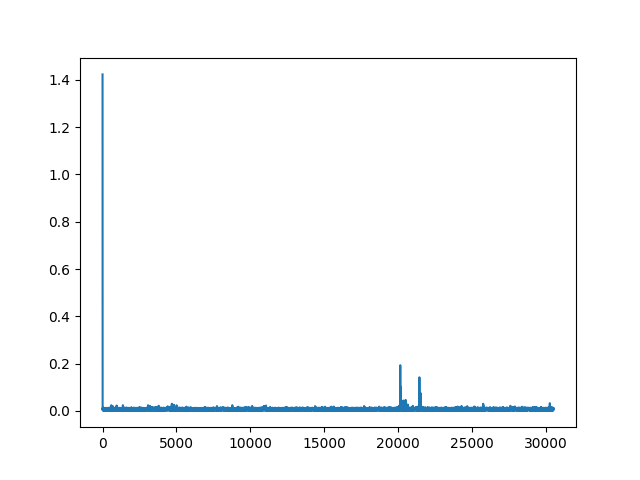
\includegraphics[scale=0.75]{incremental_times.png}
    \centering
    \caption{Per-tree wall time for computing species trees along a sequence}
    \label{fig:incremental_times}
\end{figure}

% TODO
I think this would look much better as trees per second, but this was easier
for late-night me. Also none of these graphs have axes labels.

It is worth noting that this algorithm can be used very broadly, but is optimized
for a particular use-case. The combinatorial method of ranking trees contributes
little to the overall runtime because the species trees we are ranking are very
small. More efficient indexing methods may be useful when computing on larger
numbers of species. Additionally, the higher the correlation between trees the
better the gains from using an incremental approach. Current inference methods
like \tsinfer{} can generate succinct tree sequences from variant data, but might
not achieve the compression exhibited in simulated tree sequences and thus
are slower to compute on. Nevertheless, this does mean that improvements in
inference technology have a compounding effect on the speed and accuracy
at which incremental algorithms, such as this one, operate.

\end{document}
